%TC:group table 0 1
%TC:group tabular 1 1

\chapter{Evaluation}

This chapter evaluates the performance of the Prolog implementation, WebPL, in terms of execution time (Section \ref{sec:execution-time}), memory usage (Section \ref{sec:memory-usage}), and binary size (Section \ref{sec:binary-size}), and compares it to existing Prolog implementations for the Web. Then, factors contributing to the performance differences are explored, and possible improvements to SWI-Prolog are described (Section \ref{sec:swi-prolog-optimisation}). Finally, the use of the Rust programming language is evaluated (Section \ref{sec:rust-evaluation}).

\section{Benchmark Programs}

To evaluate the performance of the Prolog implementation, a subset of the SWI-Prolog benchmark suite \cite{wielemakerSWIPrologbenchmarksuite2010}, itself derived from a collection of widely-used Prolog benchmarks \cite{haygoodPrologBenchmarkSuite1989}, was selected. This consisted of 16 benchmarks, excluding the 19 which use features not supported in WebPL.

The benchmarks selected for this evaluation cover a range of tasks, including parsing natural language, symbolic differentiation, list manipulation, arithmetic, and solving puzzles such as the 8-Queens problem. The full benchmark suite is detailed in Appendix \ref{appendix:benchmarks}.

\section{Execution Time}

\label{sec:execution-time}

The implementation-agnostic TypeScript interface, developed as part of the browser-based development environment (Section \ref{sec:prolog-interface}), was further used to build an in-browser benchmarking tool.

Each benchmark was initially run up to 20 times or for 100ms, whichever was shorter, to populate the cache. Then, during the measurement phase, each benchmark was run at least 10 more times, for a maximum of 1000 runs or 5 seconds of benchmarking. The execution time of each run was measured using the browser's \texttt{performance.now()} function, which provides high-resolution timestamps. However, high-resolution timestamps are only available in \emph{secure contexts} for security reasons \cite{sanchez-rolaClockClockTimeBased2018}, so the benchmarking tool was hosted on a local server configured to use HTTPS.

Benchmarks were run in Chrome 134 on a MacBook Pro with an Apple M3 Pro chip and 18GB of RAM, running macOS 15.3 (Sequoia).

\subsection{Comparison of Prolog Implementations}

\label{sec:prolog-comparison}

Table \ref{tab:chrome-time} shows the median execution time of each benchmark for each implementation tested.

\begin{table}[H]
\centering
\setstretch{1}
\begin{tabular}{llllll}
\addlinespace\hline\addlinespace
Benchmark & WebPL & WebPL+GC & SWI & Trealla & Tau \\
\addlinespace\hline\addlinespace
chat\_parser  & \green{17.22}  &  18.51  &  74.44  &  26.90  &  1610.90  \\
crypt        &   0.64  &   \green{0.63}  &   3.00  &   3.62  &   120.77  \\
derive       &   0.29  &   \green{0.28}  &   1.20  &   0.45  &    13.25  \\
divide10     &   0.27  &   \green{0.24}  &   1.08  &   0.39  &    12.99  \\
fib          &   \green{4.84}  &   7.41  &   9.72  &   5.08  &  3040.73  \\
log10        &   \green{0.27}  &   \green{0.27}  &   1.08  &   0.41  &    13.40  \\
mu           &   \green{0.34}  &   0.36  &   1.32  &   0.62  &    15.03  \\
nreverse     &   \green{0.29}  &   0.38  &   0.65  &   0.40  &    17.28  \\
ops8         &   0.28  &   \green{0.27}  &   1.10  &   0.46  &    13.18  \\
poly\_10      &   \green{5.48}  &  16.98$^*$  &  19.31  &   6.45  &  3481.89  \\
qsort        &   \green{0.32}  &   0.38  &   0.84  &   0.55  &    18.12  \\
queens\_8     &   \green{6.49}  &   7.30  &  17.87  &   8.38  &   267.43  \\
query        &  \green{0.77}  &   0.82  &   2.68  &   1.26  &    20.31  \\
tak          &  \green{15.33}  &  38.56$^*$  &  28.20  &  27.96  & 26691.83  \\
times10      &   \green{0.27}  &   \green{0.27}  &   1.14  &   0.57  &    12.88  \\
zebra        &   3.16  &   \green{3.13}  &   7.82  &   9.76  &   901.52  \\
\addlinespace\hline\addlinespace
\end{tabular}
\caption{Execution time of benchmarks (milliseconds)}
\label{tab:chrome-time}
\end{table}

\vspace*{-1.5em}

Unexpectedly, the results show that WebPL is faster than all other Prolog implementations tested in every benchmark without garbage collection, and all but two when garbage collection is enabled (marked with a *). Section \ref{sec:swi-prolog-optimisation} explores why this is the case, and how some modifications to the build process for SWI-Prolog can make its execution time more competitive.

\begin{figure}[H]
\centering
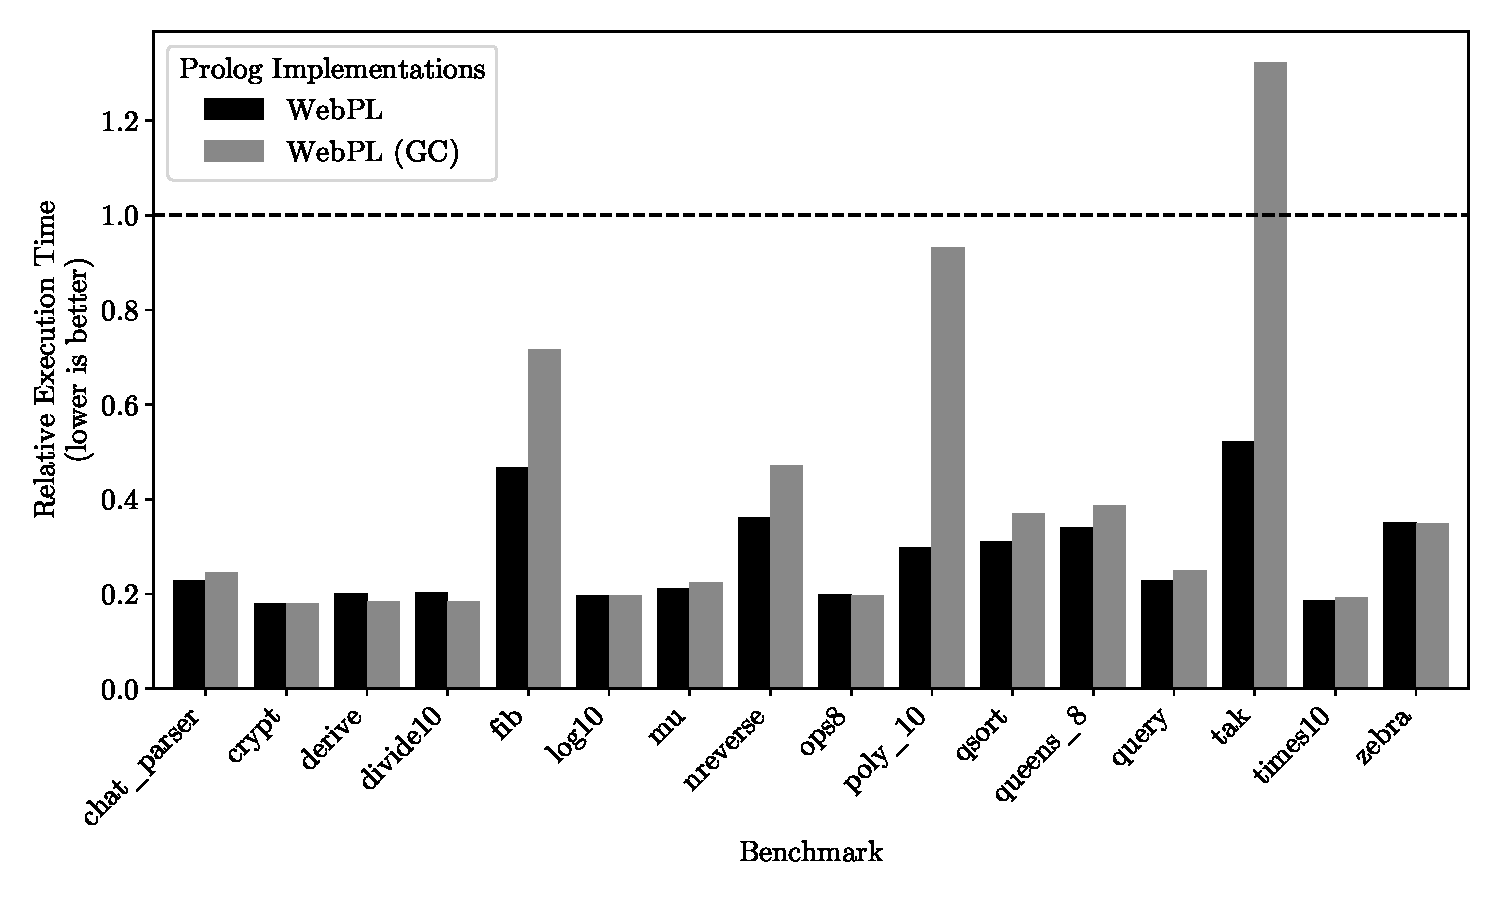
\includegraphics[width=0.8\textwidth]{relative_performance.pdf}
\caption{Execution time of benchmarks relative to SWI-Prolog}
\label{fig:relative-performance}
\end{figure}

Figure \ref{fig:relative-performance} shows the execution time of WebPL, relative to SWI-Prolog, based on the same data as Table \ref{tab:chrome-time}.

This reveals that for three benchmarks, \texttt{fib}, \texttt{poly\_10}, and \texttt{tak}, enabling garbage collection has a significant impact on performance, increasing execution time by 53\%, 210\%, and 152\% respectively. These benchmarks are the most memory-intensive, so garbage collection runs more frequently, leading to significantly decreased performance.

The WebPL garbage collection scheduler invokes the garbage collector whenever heap utilisation exceeds a certain threshold (by default, 90\%). If this does not reduce heap utilisation below the threshold, garbage collection is not invoked again until the heap has been resized, which occurs when the heap is full, and the threshold met again. In addition, there is a timeout between garbage collections to avoid invoking the garbage collector too frequently.

This is a more aggressive strategy than that of SWI-Prolog, which does not consider the allocated size of the heap when deciding when to invoke the garbage collector, instead considering the used size of the heap at the last garbage collection\footnote{\url{https://www.swi-prolog.org/pldoc/man?section=gc}}. Therefore, SWI-Prolog is less conservative of memory (Section \ref{sec:memory-usage}), and may end up resizing the heap unnecessarily, but avoids the performance penalty of frequent garbage collections.

\section{Memory Usage}

\label{sec:memory-usage}

A notable criticism of existing Prolog implementations for the Web is their high memory usage (Section \ref{sec:motivation}).

Two approaches were taken in evaluating memory usage. The browser's \texttt{performance.memory} API was used to measure the memory usage of a browser tab running the Prolog interpreter (Section \ref{sec:web-page-memory-usage}). However, this also includes the size of the WebAssembly binary, located in the memory of the browser tab. The Prolog implementation's own memory usage statistics were therefore also used, but this is only available in WebPL and SWI-Prolog (Section \ref{sec:prolog-heap-usage}).

\subsection{Web Page Memory Usage}

\label{sec:web-page-memory-usage}

To evaluate the memory usage of each Prolog implementation for each benchmark, a Python script using the Selenium browser automation library was developed. For each implementation and each benchmark, the script starts a new browser instance, loads the implementation and benchmark, runs the benchmark once, and measures the memory usage of the tab using \texttt{performance.memory}. As memory used by WebAssembly cannot be freed, the resulting measurement is the peak memory usage during the execution of the benchmark, shown in Table \ref{tab:chrome-memory}.

\begin{table}[H]
\centering
\setstretch{1}
\begin{tabular}{llllll}
\addlinespace\hline\addlinespace
Benchmark & WebPL & WebPL+GC & SWI & Trealla & Tau \\
\addlinespace\hline\addlinespace
chat\_parser & 6.02 & \green{5.58} & 36.57 & 26.05 & 83.05 \\
crypt & \green{4.90} & \green{4.90} & 36.71 & 25.10 & 29.72 \\
derive & \green{4.90} & \green{4.90} & 36.95 & 25.09 & 5.71 \\
divide10 & \green{4.90} & \green{4.90} & 36.45 & 25.09 & 5.46 \\
fib & 36.77 & \green{5.33} & 36.20 & 31.78 & 679.96 \\
log10 & \green{4.90} & \green{4.90} & 36.70 & 25.09 & 5.46 \\
mu & \green{4.90} & \green{4.90} & 36.45 & 25.09 & 5.96 \\
nreverse & \green{4.89} & \green{4.89} & 36.45 & 25.21 & 9.46 \\
ops8 & \green{4.90} & \green{4.90} & 36.45 & 25.09 & 5.46 \\
poly\_10 & 36.78 & \green{5.22} & 36.71 & 35.84 & 227.97 \\
qsort & \green{4.89} & 4.90 & 36.20 & 25.22 & 7.03 \\
queens\_8 & \green{4.90} & \green{4.90} & 36.46 & 25.10 & 69.47 \\
query & \green{4.90} & \green{4.90} & 36.71 & 25.33 & 5.72 \\
tak & 133.39 & \green{36.89} & 41.01 & 87.20 & 3186.35 \\
times10 & \green{4.90} & \green{4.90} & 36.45 & 25.09 & 5.46 \\
zebra & \green{4.90} & \green{4.90} & 36.45 & 25.10 & 104.97 \\
\addlinespace\hline\addlinespace
\end{tabular}
\caption{Memory usage of benchmarks (megabytes)}
\label{tab:chrome-memory}
\end{table}

WebPL shows the lowest memory usage for all benchmarks with garbage collection enabled. However, the variance of memory usage across benchmarks is very small due to the often much larger binary size being included in the memory of the browser tab. To better evaluate the memory usage of the Prolog implementations themselves, another approach was taken.

\subsection{Prolog Heap Usage}

\label{sec:prolog-heap-usage}

WebPL, like SWI-Prolog, provides a built-in \texttt{statistics/2} predicate to access statistics about the execution. One such statistic is the allocated size of the Prolog heap. By using this predicate at the end of the query to be benchmarked, the memory usage of the Prolog implementation itself can be measured. Figure \ref{fig:heap-usage} shows the allocated heap size of WebPL with garbage collection enabled for each benchmark, relative to that of SWI-Prolog.

\begin{figure}[t]
\centering
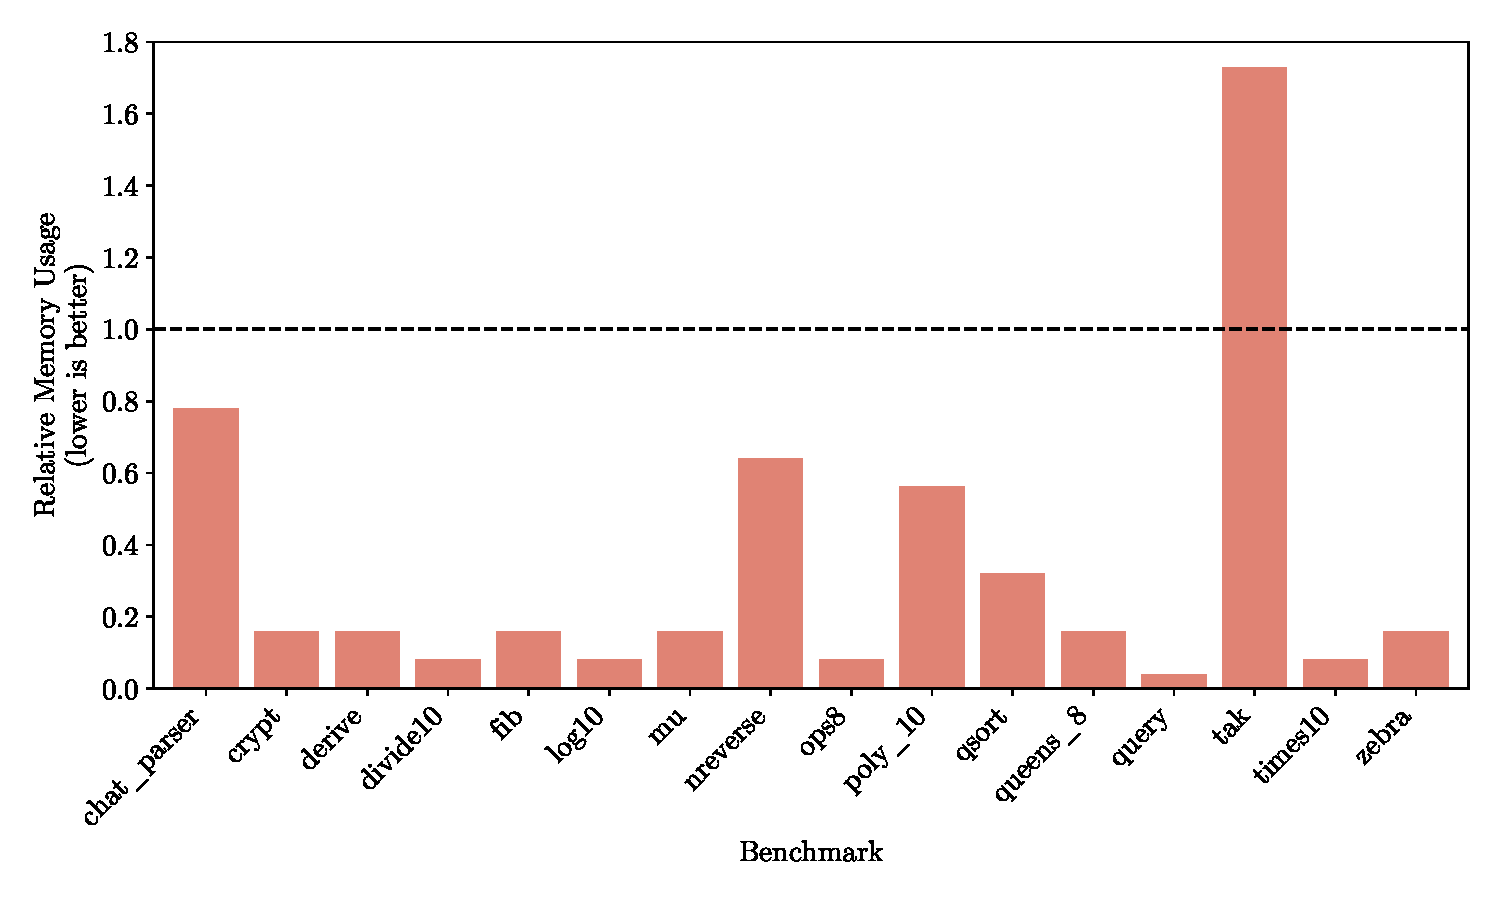
\includegraphics[width=0.8\textwidth]{relative_memory_builtin.pdf}
\caption{Allocated heap size relative to SWI-Prolog}
\label{fig:heap-usage}
\end{figure}

For some benchmarks, WebPL uses much less memory than SWI-Prolog. This is because SWI-Prolog pre-allocates a fixed amount of memory for the heap to avoid the overhead of doing so during execution, while WebPL does not pre-allocate any memory, instead doubling the size of the heap each time it gets full. As a result, WebPL never allocates more than twice the memory it needs.

For other benchmarks, WebPL uses only slightly less memory to SWI-Prolog. Only in the case of the \texttt{tak} benchmark does WebPL use more. These are the more memory-intensive benchmarks, possibly indicating that, in the limit, SWI-Prolog is more memory efficient. The use of the Rust programming language for WebPL limits the memory usage optimisations that can be made (Section \ref{sec:rust-evaluation}).

\section{Binary Size}

\label{sec:binary-size}

Another important consideration for any web application is how much data needs to be downloaded to the client. Unlike native applications, which are downloaded once and run locally, web applications are usually loaded from the server every time the client visits the page. Therefore, the size of the application can have a significant impact on the time it takes to load the page, especially on mobile devices with slower connections. This is a common weakness of WebAssembly applications, as WebAssembly binaries can be large, often due to the inclusion of libraries, such as \texttt{libc}, which, unlike in native applications, cannot be dynamically linked.

Table \ref{tab:binary-size} shows the size of the WebAssembly binary (for WebPL, SWI-Prolog, and Trealla Prolog) or the JavaScript bundle (for Tau Prolog) for each Prolog implementation.

\begin{table}[H]
\centering
\begin{tabular}{ll}
\addlinespace\hline\addlinespace
Implementation & Binary/Bundle Size \\
\addlinespace\hline\addlinespace
WebPL & 0.84 MB \\
SWI-Prolog & 7.95 MB \\
Trealla Prolog & 4.48 MB \\
Tau Prolog & \green{0.57 MB} \\
\addlinespace\hline\addlinespace
\end{tabular}
\caption{Binary/bundle size of Prolog implementations (megabytes)}
\label{tab:binary-size}
\end{table}

While Tau Prolog, written in JavaScript, is the smallest, WebPL is the only WebAssembly implementation smaller than 1MB, and is only 48\% larger than Tau Prolog, a significant improvement over SWI-Prolog and Trealla Prolog. Section \ref{sec:binary-size-opt} explores why SWI-Prolog is so large, and how its size can be reduced.

\section{SWI-Prolog Optimisation}

\label{sec:swi-prolog-optimisation}

Given the unexpectedly poor performance of industry-standard SWI-Prolog in both execution time and binary size, I explored why this may be, and made some optimisations.

\subsection{Profiling SWI-Prolog}

As identified in Section \ref{sec:prolog-comparison}, WebPL's execution time is significantly faster than that of SWI-Prolog. To explore why this is the case, I profiled the execution of the \texttt{queens\_8} benchmark in SWI-Prolog using Chrome DevTools. Figure \ref{fig:swi-prolog-profile} shows a screenshot of the stack chart.

\begin{figure}[H]
\centering
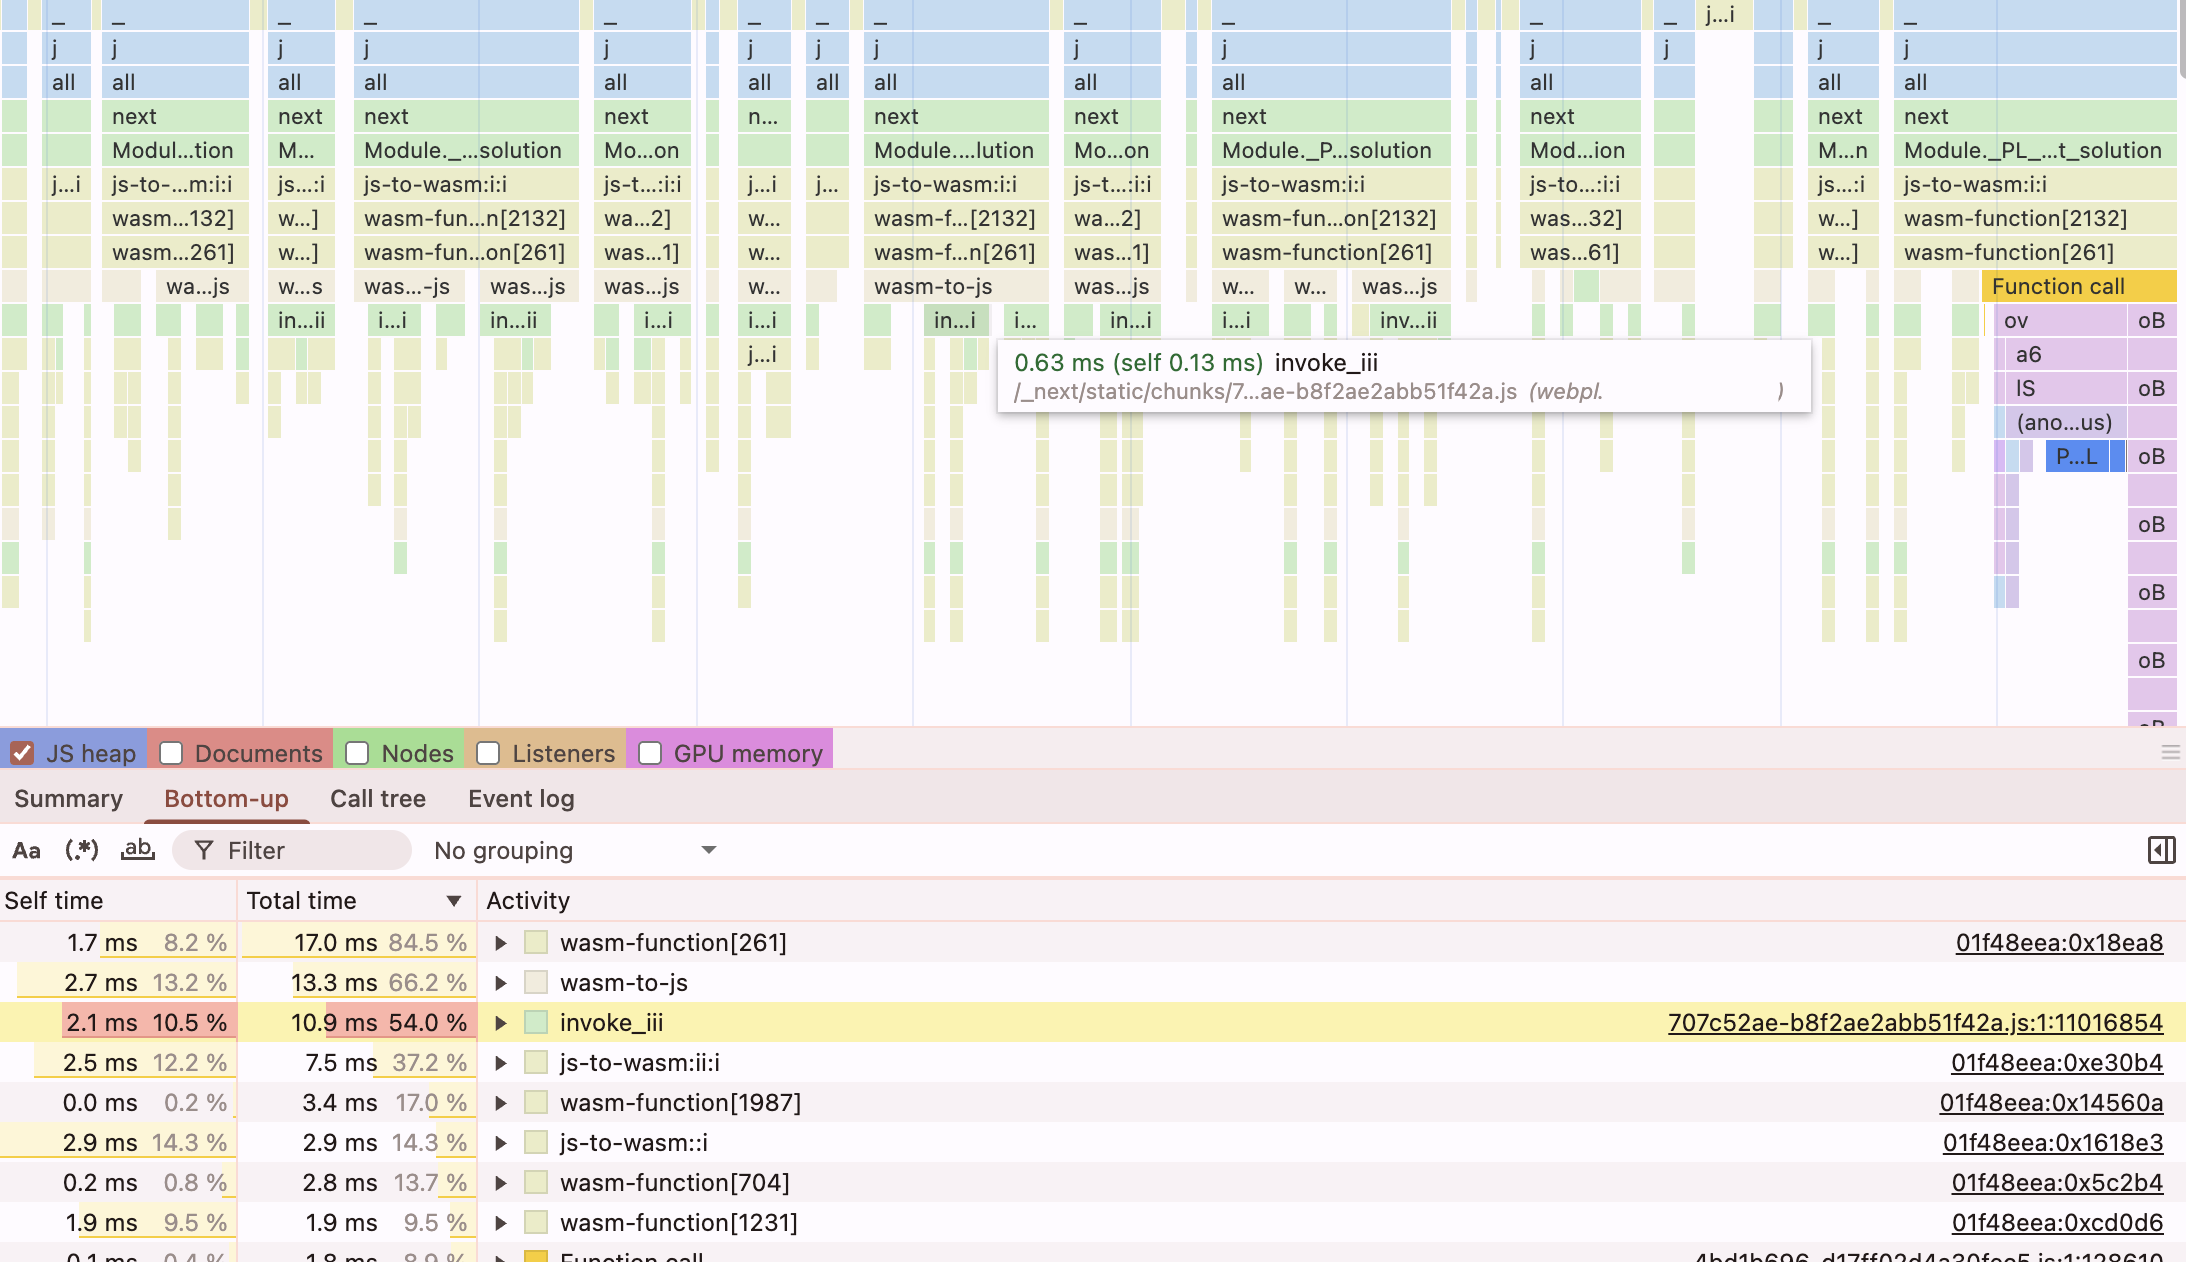
\includegraphics[width=0.8\textwidth]{08evaluation_swiprofiling.png}
\caption{Stack chart of SWI-Prolog execution}
\label{fig:swi-prolog-profile}
\end{figure}

This revealed that a great deal of time is spent crossing the boundary between WebAssembly and JavaScript code, in particular calling the \texttt{invoke\_iii} JavaScript function from WebAssembly, which promptly calls back into WebAssembly code. This function is generated by Emscripten, the compiler used to compile SWI-Prolog to WebAssembly, and is shown in Figure \ref{fig:invoke-iii}.

\begin{figure}[H]
\centering
\begin{minted}{javascript}
function invoke_iii(A, g, I) {
    var C = stackSave();
    try {
        return getWasmTableEntry(A)(g, I)
    } catch (A) {
        if (stackRestore(C),
        A !== A + 0)
            throw A;
        _setThrew(1, 0)
    }
}
\end{minted}
\caption{The \texttt{invoke\_iii} JavaScript function}
\label{fig:invoke-iii}
\end{figure}

WebAssembly does not have a built-in exception mechanism, so Emscripten uses JavaScript exceptions instead. The \texttt{invoke\_iii} function is used to invoke a WebAssembly function that might raise an exception, and perform the necessary stack manipulation to jump back to the WebAssembly code that handles the exception if one is raised. This comes at the performance cost of crossing the JavaScript-WebAssembly boundary not only when raising an exception, but also when calling any function that might do so.

SWI-Prolog is written in C, so it does not itself use exceptions. However, it supports Prolog exceptions (extra-logical predicates that can be used to implement more complex control flow), and these are implemented using C \texttt{setjmp} and \texttt{longjmp} functions. Emscripten uses the same \texttt{invoke\_iii} mechanism to implement these functions.

\subsection{Experimental WebAssembly Exception Support}

While exceptions are not currently supported in WebAssembly, there is a proposal\footnote{\url{https://github.com/WebAssembly/exception-handling/blob/main/proposals/exception-handling/Exceptions.md}} to do so. This has been experimentally implemented in Chrome's V8 JavaScript engine, and can be enabled with the \texttt{--enable-experimental-webassembly-features} flag.

To evaluate the potential performance gains of this feature for SWI-Prolog, I modified the SWI-Prolog build process to enable experimental WebAssembly exception support in Emscripten and Node.js, which is used to run some SWI-Prolog tests. SWI-Prolog is built using the Docker container system, so I added the necessary flags in various places in the Dockerfile, as well as making further changes to have it build on the Arm architecture.

\vspace*{-1em}

\begin{verbatim}
-fno-exceptions -s WASM_EXNREF=1 -s SUPPORT_LONGJMP=wasm
\end{verbatim}

\vspace*{-1em}

The benchmark suite was then re-run with the modified SWI-Prolog build in Chrome with experimental WebAssembly exception support enabled. Figure \ref{fig:swi-prolog-exception} shows the execution time of WebPL and the experimental version of SWI-Prolog, relative to the original version.

\begin{figure}[H]
\centering
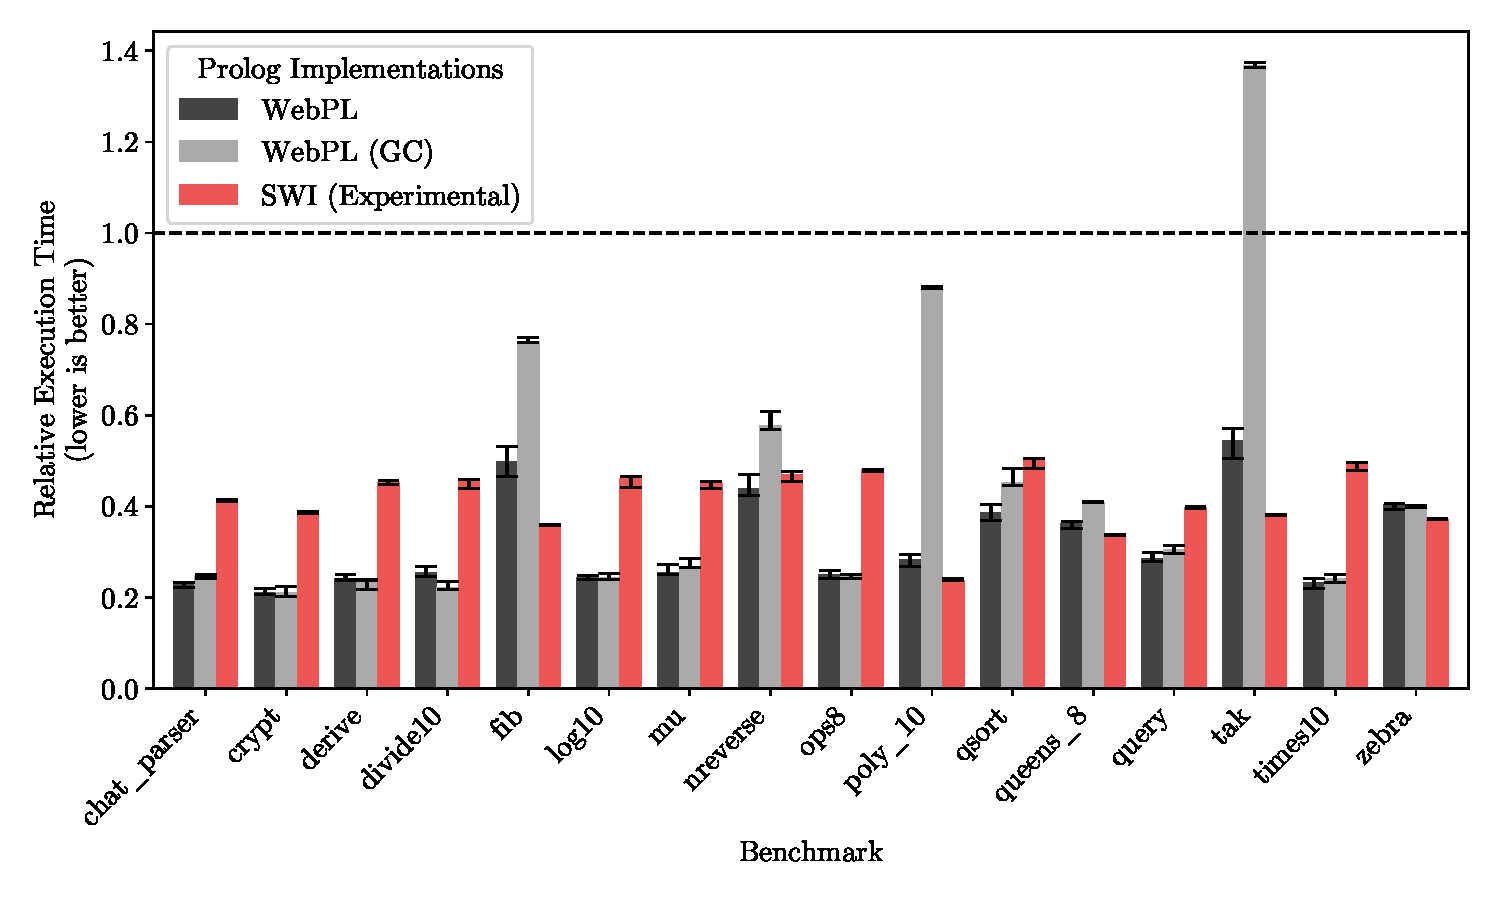
\includegraphics[width=0.8\textwidth]{relative_performance_exnref.pdf}
\caption{Execution time of benchmarks relative to SWI-Prolog}
\label{fig:swi-prolog-exception}
\end{figure}

This shows that enabling experimental WebAssembly exception support in SWI-Prolog reduces execution time by an average of around 60\%, bringing it much closer to, and in some cases surpassing, WebPL.

\subsection{Binary Size}

\label{sec:binary-size-opt}

The size of the SWI-Prolog WebAssembly binary is almost ten times larger than that of WebPL (Section \ref{sec:binary-size}). It has three distinct parts: the WebAssembly code itself (1.99 MB), various libraries (5.80 MB), and JavaScript glue code (0.16 MB). Many of the libraries are not needed in most applications, so I explored ways to build a ``minimal'' version of SWI-Prolog as a fairer comparison.

The SWI-Prolog build process provides a \texttt{-DSWIPL-PACKAGES=OFF} flag which disables the inclusion of all libraries except the standard library, reducing the size of the libraries by nearly half to 2.99 MB and the WebAssembly code to 1.23 MB. However, the WebAssembly build depends on the \texttt{clib} library to load Prolog code from a URL. Building with just this library enabled results in WebAssembly code of 1.44 MB and libraries of 3.27 MB.

This is still 0.49 MB more than building without \texttt{clib}. To avoid this 0.49 MB dependency, I rewrote part of the \texttt{wasm.pl} library in the SWI-Prolog source code to use SWI-Prolog's built-in pure-Prolog \texttt{url} library instead of \texttt{clib}, which is partially written in C.

Figure \ref{fig:binary-size} shows the size of each configuration, and compares them to WebPL.

\begin{figure}[H]
\centering
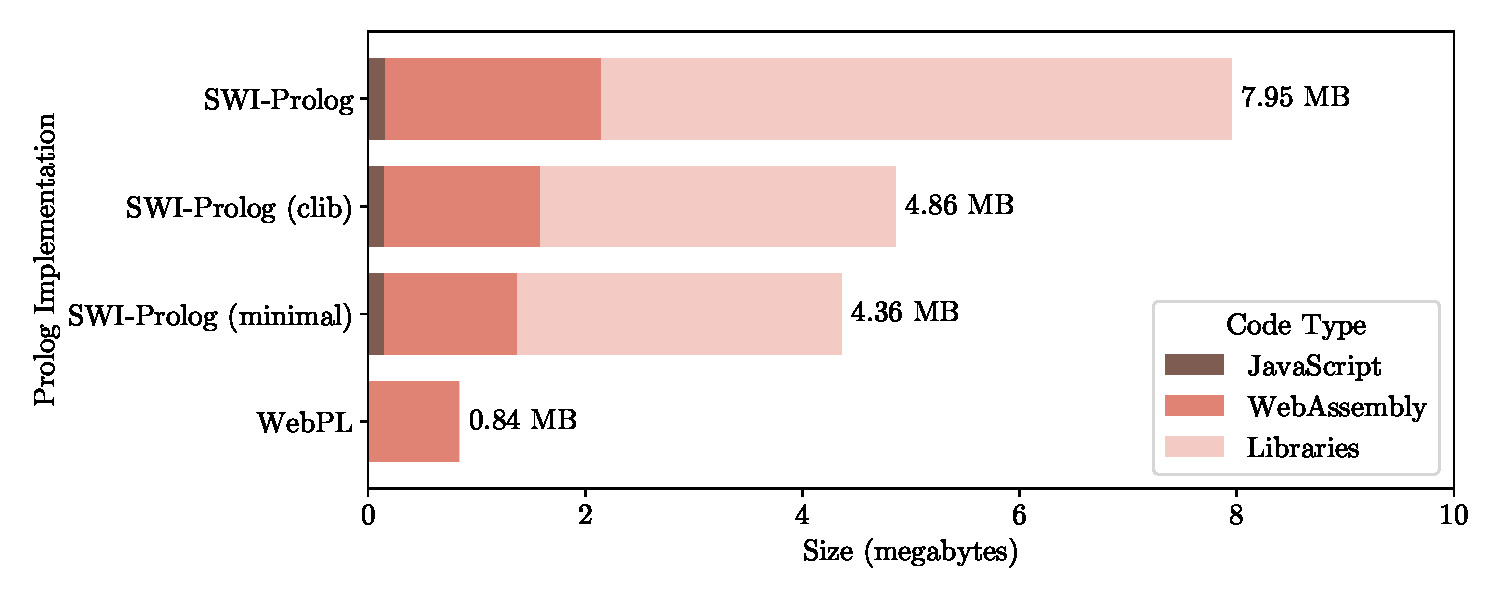
\includegraphics[width=0.8\textwidth]{binary_size.pdf}
\caption{Size of WebAssembly binaries for Prolog implementations}
\label{fig:binary-size}
\end{figure}

\vspace*{-1.5em}

Another approach explored to reduce binary size was the \texttt{wasm-opt} tool, part of the Binaryen project \cite{zakaiBinaryenhttpsgithubcom2015}, configured to optimise aggressively for size using the \texttt{-Oz} flag. However, this only reduced the size of the SWI-Prolog binary by 0.38\%, and WebPL by 0.62\%. This is likely because the compiler is already running code size optimisations by default; indeed, compiling WebPL without optimisations gives a binary size of 14.16 MB, more than 16 times larger than the optimised version.

While WebPL was built from scratch, conscious of the size of the binary, SWI-Prolog's WebAssembly port was not, and even intentionally avoided some optimisations that would have reduced its binary size in favour of keeping the port closer to the native version\footnote{\url{https://swi-prolog.discourse.group/t/wiki-discussion-swi-prolog-in-the-browser-using-wasm/5651/109}}.

\section{Rust Evaluation}

\label{sec:rust-evaluation}

WebPL is written in Rust to take advantage of its extensive support for WebAssembly and its performance (Section \ref{sec:tools}). This section explores aspects of Rust that may affect performance.

\subsection{Unsafe Rust}

Rust is known for its memory safety guarantees. Many of these are verified at compile time by the borrow checker, which enforces the ownership and borrowing rules of Rust and prevents common causes of memory errors, such as use-after-free and double-free errors. However, some checks cannot be performed at compile time, such as bounds checking, and are instead performed at runtime, at a performance cost.

Rust provides the \texttt{unsafe} keyword to bypass these checks. This is necessary for interfacing with external code that the borrow checker cannot verify, but can also be used cautiously to improve performance.

WebPL represents the heap as an array of fixed-size terms (Section \ref{sec:memory-layout}), so indexing into the heap involves a bounds check. By using \texttt{unsafe} to bypass this check, the performance of the Prolog interpreter may improve.

Figure \ref{fig:unsafe} shows the relative execution time of each benchmark without bounds-checking, compared to the original version of WebPL.

\begin{figure}[H]
\centering
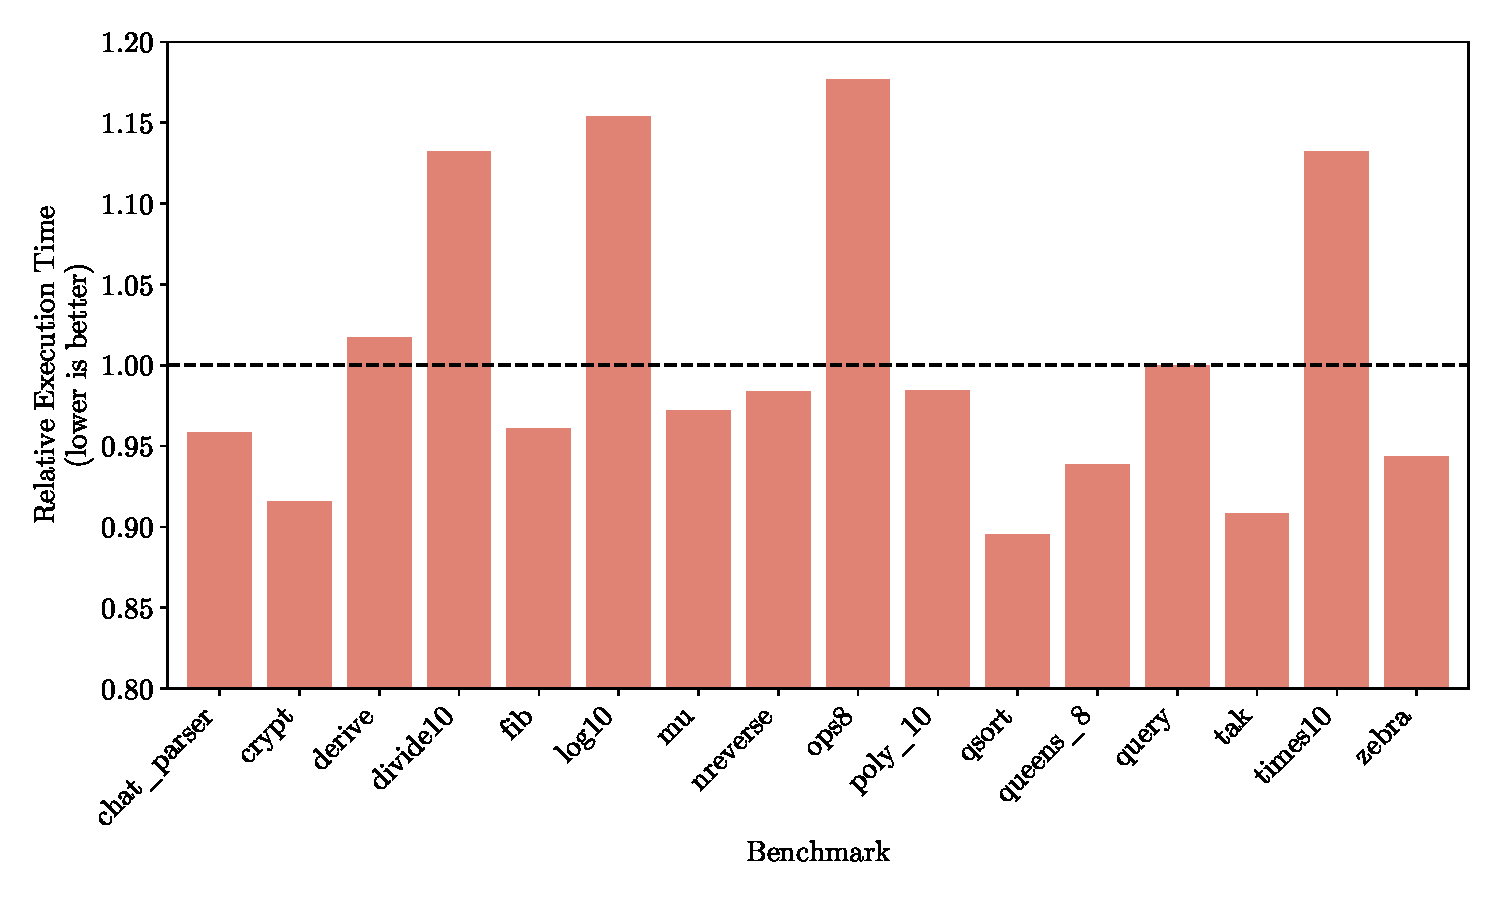
\includegraphics[width=0.8\textwidth]{relative_performance_unsafe.pdf}
\caption{Execution time of benchmarks relative to WebPL}
\label{fig:unsafe}
\end{figure}

The results are not consistent across benchmarks -- the more heavyweight benchmarks, like \texttt{fib}, \texttt{queens\_8}, and \texttt{tak}, show an improvement of up to 10\% lower execution time, while the lighter benchmarks, like \texttt{divide10}, \texttt{ops8}, and \texttt{times10}, show a degradation of up to 20\% higher execution time. This is likely due to the fact that the overhead of bounds-checking is negligible for lightweight benchmarks, and using unsafe code reduces the compiler's optimisation opportunities.

For this reason, alongside that Rust discourages the use of unsafe code, unsafe code was not used in WebPL.

\subsection{Memory Layout}

Using a Rust \texttt{enum} to represent terms leaves their layout in memory up to the compiler, which may use more memory than necessary to represent the term. The exact memory layout in WebAssembly can be inspected using experimental Rust compiler flags:

\begin{verbatim}
$ cargo +nightly rustc --target wasm32-unknown-unknown -- -Zprint-type-sizes
\end{verbatim}

Figure \ref{fig:memory-layout-wasm} shows the memory layout of an integer atom term and a variable term in WebAssembly. This reveals a lot of wasted space: flags \texttt{shunted} and \texttt{attributed} use a byte each, and the tag indicating the type of the term uses 4 bytes, even though one would suffice.

\begin{figure}[H]
\centering
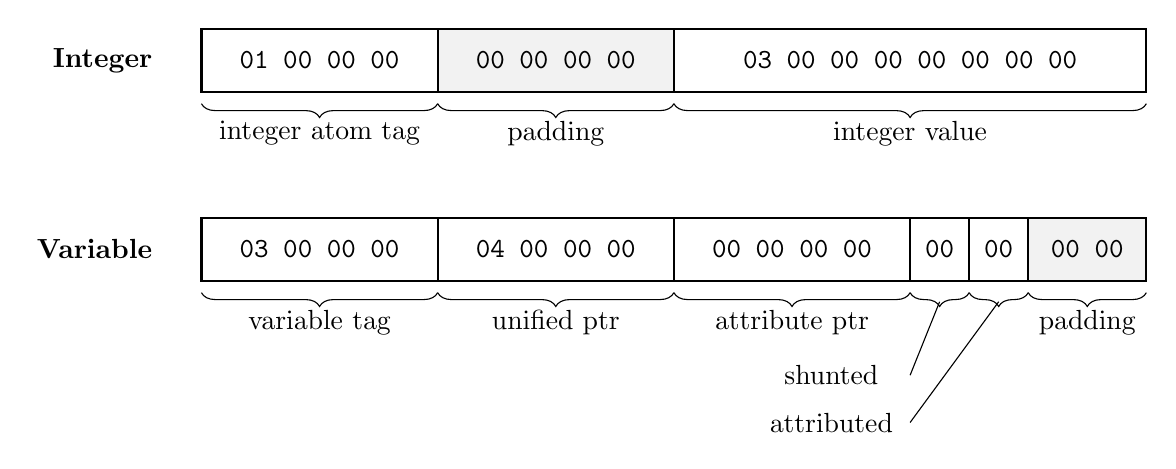
\begin{tikzpicture}[yscale=0.8]

\fill[thick, black!5] (3,0) rectangle (6,1);
\draw[thick] (0,0) rectangle (12,1);

\draw[thick] (3,0) -- (3,1);
\draw[thick] (6,0) -- (6,1);

\node at (1.5,0.5) {\texttt{01 00 00 00}};
\node at (4.5,0.5) {\texttt{00 00 00 00}};
\node at (9,0.5) {\texttt{03 00 00 00 00 00 00 00}};

\draw [decorate,decoration={brace,amplitude=5pt,mirror,raise=1ex}] (0,0) -- (3,0) node[midway,yshift=-1.5em]{integer atom tag};
\draw [decorate,decoration={brace,amplitude=5pt,mirror,raise=1ex}] (3,0) -- (6,0) node[midway,yshift=-1.5em]{padding};
\draw [decorate,decoration={brace,amplitude=5pt,mirror,raise=1ex}] (6,0) -- (12,0) node[midway,yshift=-1.5em]{integer value};

\fill[thick, black!5] (10.5,-3) rectangle (12,-2);
\draw[thick] (0,-3) rectangle (12,-2);

\draw[thick] (3,-3) -- (3,-2);
\draw[thick] (6,-3) -- (6,-2);
\draw[thick] (9,-3) -- (9,-2);
\draw[thick] (9.75,-3) -- (9.75,-2);
\draw[thick] (10.5,-3) -- (10.5,-2);

\node at (1.5,-2.5) {\texttt{03 00 00 00}};
\node at (4.5,-2.5) {\texttt{04 00 00 00}};
\node at (7.5,-2.5) {\texttt{00 00 00 00}};
\node at (9.375,-2.5) {\texttt{00}};
\node at (10.125,-2.5) {\texttt{00}};
\node at (11.25,-2.5) {\texttt{00 00}};

\draw [decorate,decoration={brace,amplitude=5pt,mirror,raise=1ex}] (0,-3) -- (3,-3) node[midway,yshift=-1.5em]{variable tag};
\draw [decorate,decoration={brace,amplitude=5pt,mirror,raise=1ex}] (3,-3) -- (6,-3) node[midway,yshift=-1.5em]{unified ptr};
\draw [decorate,decoration={brace,amplitude=5pt,mirror,raise=1ex}] (6,-3) -- (9,-3) node[midway,yshift=-1.5em]{attribute ptr};
\draw [decorate,decoration={brace,amplitude=5pt,mirror,raise=1ex}] (9,-3) -- (9.75,-3) node[midway,yshift=-1.5em]{};
\draw [decorate,decoration={brace,amplitude=5pt,mirror,raise=1ex}] (9.75,-3) -- (10.5,-3) node[midway,yshift=-1.5em]{};
\draw [decorate,decoration={brace,amplitude=5pt,mirror,raise=1ex}] (10.5,-3) -- (12,-3) node[midway,yshift=-1.5em]{padding};

\node (S) at (8,-4.5) {shunted};
\node (A) at (8,-5.25) {attributed};

\draw (9,-4.5) -- (9.375,-3.333);
\draw (9,-5.25) -- (10.125,-3.333);

\node at (-0.5,0.5) [anchor=east] {\bf Integer};
\node at (-0.5,-2.5) [anchor=east] {\bf Variable};

\end{tikzpicture}
\caption{Memory layout of Prolog terms in WebAssembly}
\label{fig:memory-layout-wasm}
\end{figure}

Padding is used by the compiler to ensure that heap terms are aligned to 8-byte boundaries, which is sensible for performance reasons, and strictly necessary on some architectures. However, this is not the case in WebAssembly, as the WebAssembly specification explicitly states that unaligned accesses must be allowed \cite{rossbergWebAssemblyCoreSpecification2022}, although underlying hardware constraints may mean that unaligned accesses are slower.

Therefore, if a more compact representation of terms were used, consolidating the tag and flags into a single byte and removing padding, the size of each term could be reduced from 16 bytes to 9 bytes, reducing heap usage by 44\%. It is possible that maintaining some alignment would still be a worthwhile trade-off, perhaps 4-byte alignment, but this would require more investigation.

Since Rust does not support this level of control over the memory layout without using unions and unsafe code, a pattern that is far from idiomatic, this is not a change that was easily possible to implement in WebPL. However, if the project were to be rewritten in a language like C++, this could be a worthwhile optimisation to explore.